\tikzset{
  basic/.style  = {draw, text width=2cm, rectangle},
  root/.style   = {basic, rounded corners=2pt, thin, align=center, fill=gray!30},
  level 2/.style = {basic, rounded corners=2pt, thin, align=center, text width=6em},
  level 3/.style = {basic, dashed, align=center, text width=4.5em, fill=gray!30},
  level 4/.style = {basic, rounded corners=6pt, thin, align=center}
}

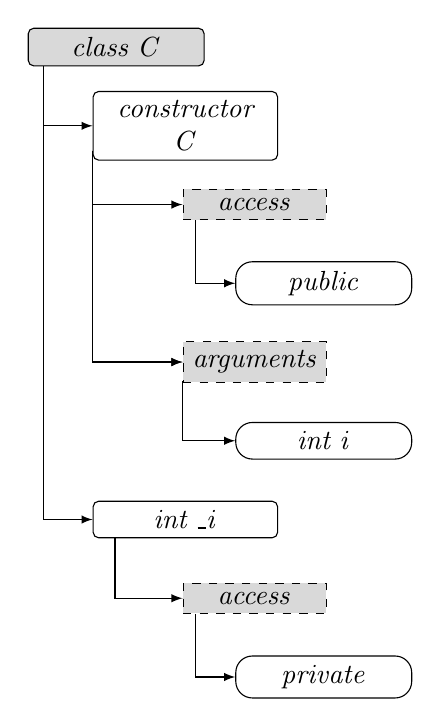
\begin{tikzpicture}[
  level 1/.style={sibling distance=40mm},
  edge from parent/.style={->,draw},
  >=latex, level distance=1.8cm]

\node[root] (c2) {\textit{class C}};

% The second level, relatively positioned nodes
\begin{scope}[every node/.style={level 2}]
\node [below of = c2, xshift=25pt] (c21) {\textit{constructor C}};
\end{scope}

\begin{scope}[every node/.style={level 3}]
\node [below of = c21, xshift=25pt] (c212) {\textit{access}};
\end{scope}

\begin{scope}[every node/.style={level 4}]
\node [below of = c212, xshift=25pt] (c2121) {\textit{public}};
\end{scope}

\begin{scope}[every node/.style={level 3}]
\node [below of = c2121, xshift=-25pt] (c211) {\textit{arguments}};
\end{scope}

\begin{scope}[every node/.style={level 4}]
\node [below of = c211, xshift=25pt] (c2111) {\textit{int i}};
\end{scope}

\begin{scope}[every node/.style={level 2}]
\node [below of = c2111, xshift=-50pt] (c22) {\textit{int \_i}};
\end{scope}

\begin{scope}[every node/.style={level 3}]
\node [below of = c22, xshift=25pt] (c221) {\textit{access}};
\end{scope}

\begin{scope}[every node/.style={level 4}]
\node [below of = c221, xshift=25pt] (c2211) {\textit{private}};
\end{scope}

\foreach \value in {1,...,2}
  \draw[->] (c2.195) |- (c2\value.west);

\foreach \value in {1,...,2}
 \draw[->] (c21.195) |- (c21\value.west);

\draw[->] (c21.195) |- (c211.west);
\draw[->] (c211.195) |- (c2111.west);
\draw[->] (c212.195) |- (c2121.west);

\draw[->] (c22.195) |- (c221.west);
\draw[->] (c221.195) |- (c2211.west);

\end{tikzpicture}